\section{Prototipagem}

Nesta fase de conceção da interface do utilizador, começou-se a dar mais importantia as questões estéticas. Criou-se então protótipos com recurso a \emph{HTML CSS e JavaScript}. Houve também uma nova avaliação à usabilidade da mesma.

Quanto a adaptação da interface à ecrãs de diferentes tamanhos, utilizou-se o sistema de \emph{grids} do\emph{Bootstrap}, uma \emph{framework} de \emph{CSS e JavaScript}.

Na figura ~\ref{fig:proto_dash} está o protótipo correspondente à \emph{Dashboard} quando acedida a partir de um \emph{browser} num ecrã \'comum\' e na figura ~\ref{fig:proto_mobile} está o \emph{protótipo} correspondente à \emph{Dashboard} quando acedida a partir da aplicação \emph{mobile}.

\begin{figure}[ht]
\centering
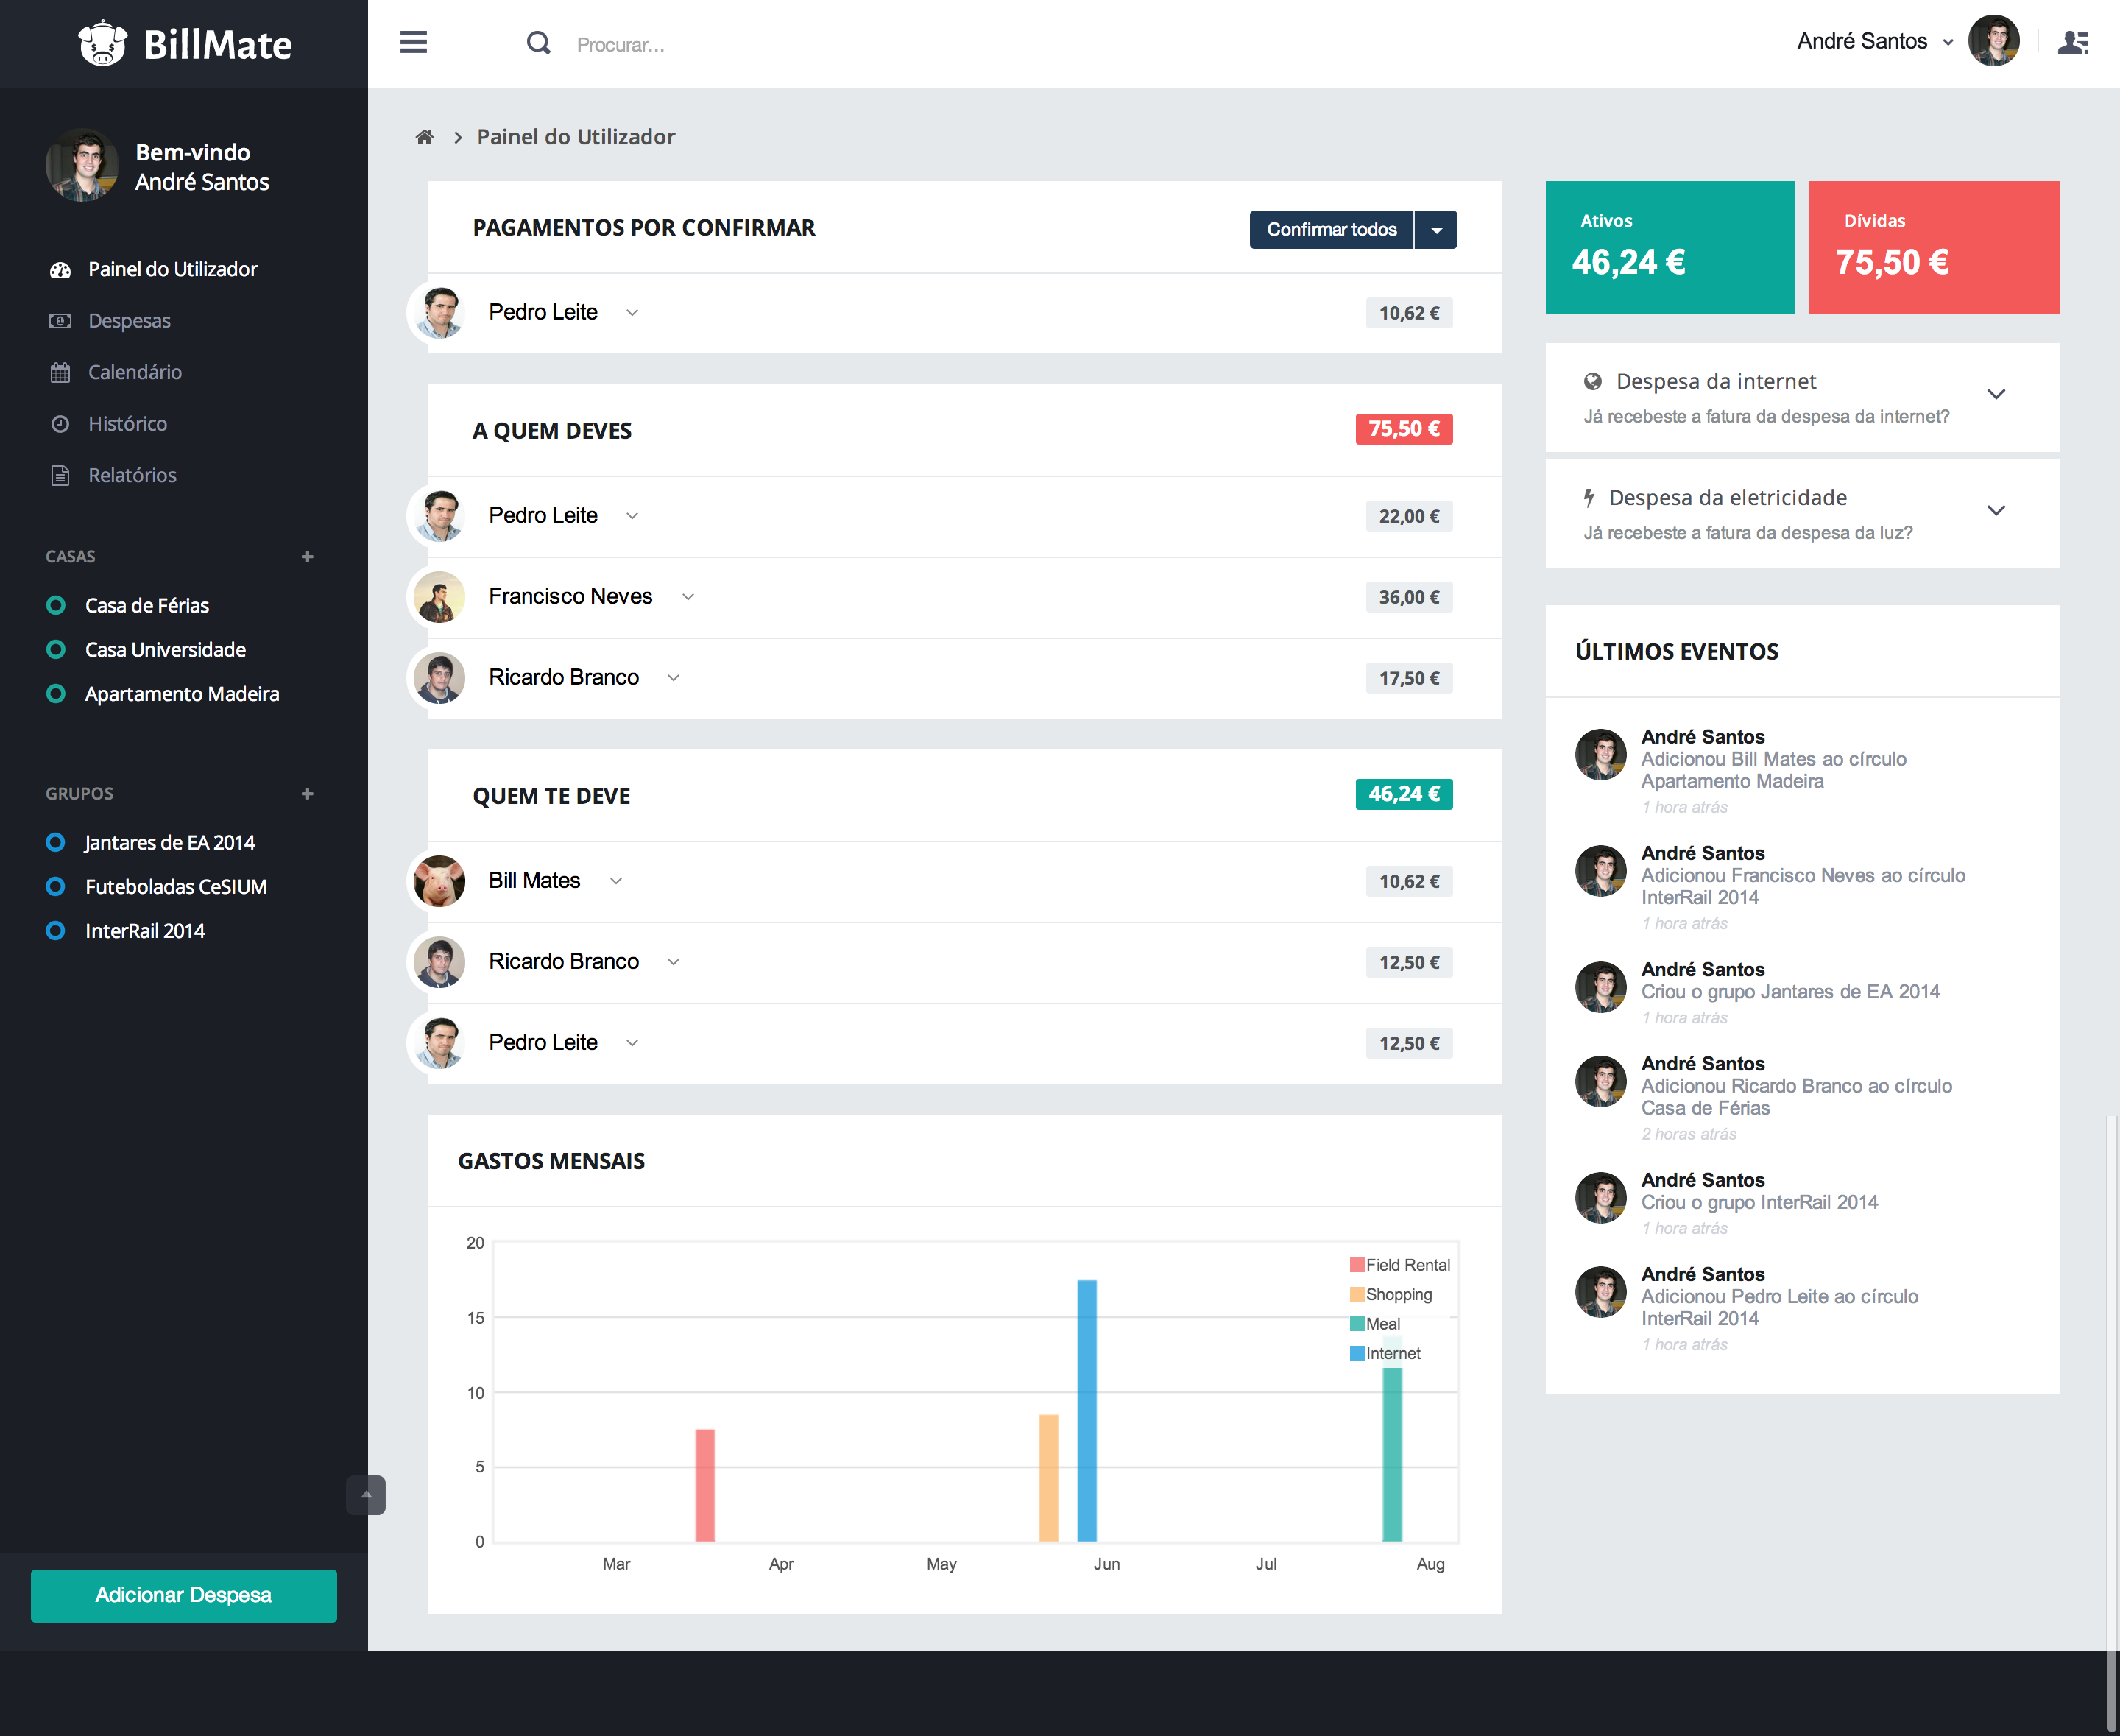
\includegraphics[width=.9\textwidth]{images/dashboardprot}
\caption{Dashboard vista a partir do \emph{browser}}
\label{fig:proto_dash}
\end{figure}


\begin{figure}[ht]
\centering
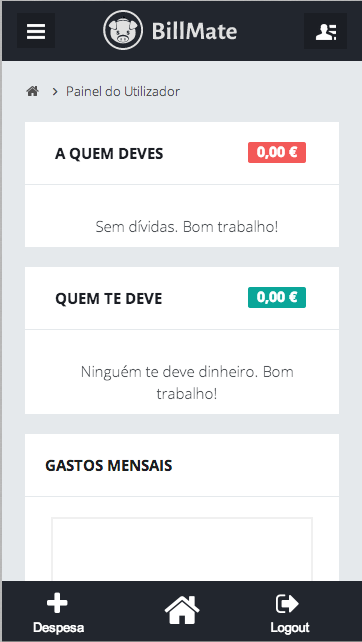
\includegraphics[width=.9\textwidth]{images/protmobile}
\caption{Dashboard vista a partir da aplicação \emph{mobile}}
\label{fig:proto_mobile}
\end{figure}
